% Project Description

\documentclass[12pt]{article}
\usepackage[letterpaper, margin=1in]{geometry}
\usepackage[utf8]{inputenc}
\usepackage{physics}
\usepackage{amsmath}
\usepackage{amssymb}
\usepackage{hyperref}
\usepackage{listings}
\usepackage{graphicx}

\begin{document}

\begin{center}
    \textbf{\Large Poisson's Spot Simulator}
\end{center}

\textbf{Group Members:}

\qquad Zhexing Zhang

\qquad Renjie Zhu

\section{Installing Required Packages}

The python modules required to run this program are,
\begin{itemize}
    \item \href{http://www.numpy.org/}{numpy}
    \item \href{https://matplotlib.org/}{matplotlib}
    \item \href{https://pypi.org/project/PyQt5/}{PyQt5}.
\end{itemize}

All three modules should have already been installed on the 
Raspberry Pi configured for PHYS 129L, but for use on 
other systems (including Windows 10, macOS and full-fledged
Linux), please run the following commands in the corresponding
command line tools.

{\fontfamily{lmtt}\selectfont 
\begin{lstlisting}
    pip3 install numpy
    pip3 install matplotlib
    pip3 install pyqt5
\end{lstlisting}
}

Due to the ARM architecture of the processor of Raspberry 
Pi 3 Model B, the above commands may not work and user 
should look for other solutions if any modules above are 
not installed. 

\section{External Hardwares}

There are no external hardwares needed for this program to
function.

\section{Program Description}

The program is a Poisson Spot Simulator using Huygens–Fresnel 
principle. According to the principle, each point on the 
light path can be seen as a secondary point light source, 
so every grid point outside the disk are used as a light 
source with same phase. The intensity of a point on the screen 
will be the superposition of the light from these points. 
The phase shifts of the points will cause interference, and 
ultimately lead to the appearance of a Poisson Spot.

The phase shifts of the light sources are caused by the 
difference of the distance between the sources and the 
point on the screen. Following this idea, distance between 
each light source and the point are calcluated as a matrix.
The matrix is then used to calculate the phases of the lights 
using exponential expression ($e^{i\theta}$, where $\theta = \frac{2 \pi l}{\lambda}$). 
The absolute value of the sum of the phases is the intensity 
of that point. 

Since the Poisson Spot is a radial symmetric plot of the 
interference pattern of light outside the disk. The intensities 
of light at different distance to the origin are calculated 
instead of looping through all the points on the x-y plane. 
The intensity function of r is then converted back to points 
on the x-y plane. Plotting the grid of points using cmap 
`gray' and the interference pattern of the 
Poisson Spot is shown. Note that the graph shows only the intensity 
but not the color of the wavelength used.

A more efficient way suggested by Professor Lipman is to use the 
complement light method. This method states that the intensity 
of a hole with same radius of the disk will show a complementary
interference pattern of the pattern of the disk. This is a 
promising method to speed up the program, but the algorithm gives
the constant intensity on the screen as complex numbers with 
unknown phases, which will ruin the plausibility of this method. 

\section{Results}

To run this program, go to the project directory and run
the following command:
{\fontfamily{lmtt}\selectfont 
\begin{lstlisting}
    $project_directory$ main.py
\end{lstlisting}
}

You will be greeted with an introduction of the program 
when you start. Press OK to go to the input interface.
A suggestion is shown on this page, but you can change 
these parameters as long as they meet the requirements
of poisson spot interference pattern. The program will
take about 10 minutes on a Raspberry Pi 3 Model B to run
and show the image. After the image is shown, 
the image will be saved as an eps
file with parameters in the filename to avoid duplication.

After the first image is shown, you can change the parameters
and compute another interference pattern using outher 
parameters. Some example images created by
this program are shown at the end of the document.

\begin{figure} [h]
    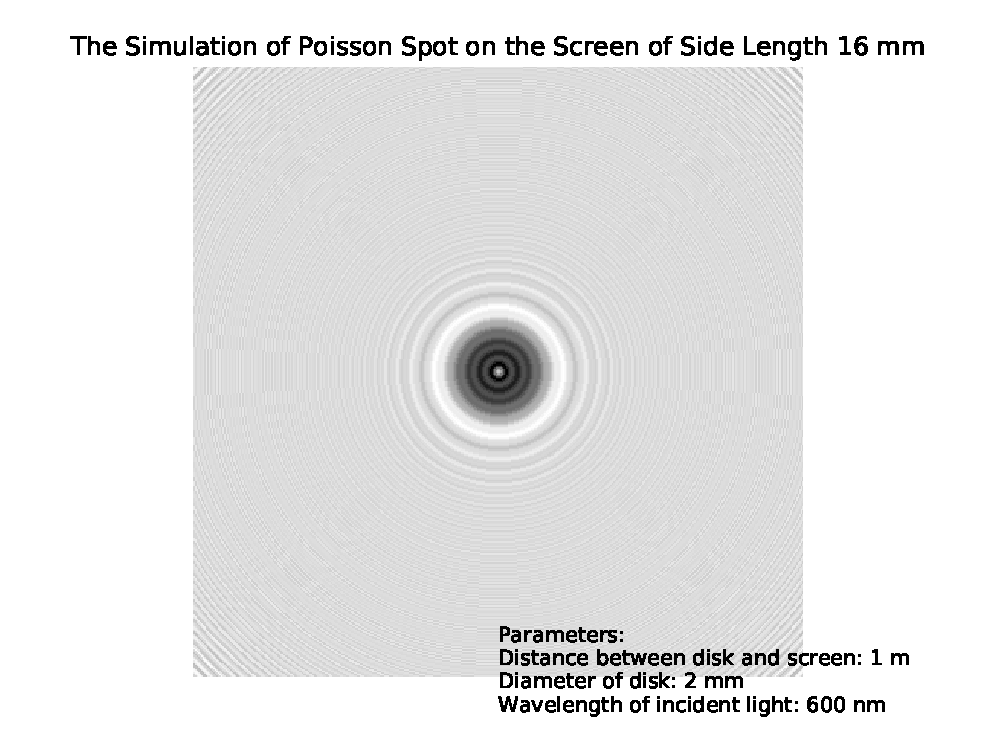
\includegraphics[width=\textwidth]{poisson_spot_1_2_600.eps}
    \caption{Example 1 with parameters shown in the figure.} 
\end{figure}

\begin{figure} [h]
    \includegraphics[width=\textwidth]{poisson_spot_1_5_700.eps}
    \caption{Example 2 with parameters shown in the figure.} 
\end{figure}

\begin{figure} [h]
    \includegraphics[width=\textwidth]{poisson_spot_2_3_450.eps}
    \caption{Example 3 with parameters shown in the figure.} 
\end{figure}

\section{Credits}

This program is divided into two main parts: GUI 
and algorithm. Renjie Zhu is responsible mainly for the 
GUI part and other user interactive parts. Zhexing Zhang 
is responsible for implementing the algorithm that 
generates a grid of resulting intensity from the diffraction.
However, extensive collaboration is the key during the
process of writing this program and is the reason this 
program works as described.

We want to thank Jiahao for testing the program 
and giving feedback about the user experience. We also
want to thank Prof. Lipman for the insight and help on the 
problems we were trying to solve.

\end{document}